%!TEX root = mainfile.tex

\section{Photometry and Colour} % (fold)
\label{sec:Photometry_Colour}
	Photometry today is used primaily with CCDs, which can convert the transmitted flux into an electric signal which can then be interpretted as a magnitude. The magnitude system used in this project was the AB magnitude system as outlined in Section~\ref{ssub:ab_magnitude}.

	In this project wide and intermediate filters have been used predominantly. A common method for making these filters is to use coloured glass which either pass all light above a certain wavelength or pass all light up to a certain wavelength, these are known as cutoff filters. A bandpass filter can be made by combining two types of coloured glass, one which will act as the low wavelength cutoff and the other as the high wavelength cutoff. Filters don't transmit 100\% of the wavelengths that are allowed to pass, and the cutoff isn't at an exact frequency. An example of this is shown in Figure ....

	To detect lyman-break galaxies the dropout method is used, which uses at least three filters to get enough spectral information to identify the object as a candidate for being a lyman break galaxy (see dropout method Section~\ref{ssub:filters_and_the_dropout_technique}). However, observing the drop due to the Gunn-Peterson effect is not enough to confirm the identities of these candidates, other observational methods need to be used to be certain the object is a lyman break galaxy and not a contaminant. One of the most effective ways of eliminating contaminants is to use the colour of the object between different filters, obtained from the photometric measurements.

    \subsection{Contaminants} %fold
    \label{sub:Contanimants}
    	\subsubsection{Sources of Contamination} % (fold)
    	\label{ssub:sources_of_contamination}
    	%Need to be one level lower, may change

		    \subsubsection*{Low Mass Stars} % (fold)
		    \label{sub:low_mass_stars}
		        These can easily be identified due to the high resolution imaging provided by JWST and Euclid. The Point-spread function (PSF) obtained will allow us to determine which sources are point-like and which are extended. We should be able to avoid significant contamination by removing any point-like sources from the results as all galaxies should have a great enough diameter.
		    % subsection low_mass_stars (end)

		    \subsubsection*{Spurious Sources} % (fold)
		    \label{sub:spurious_sources}
		        By stipulating that we will be requiring detections in two bands the influence of spurious sources will be negligible. Finding detections in 2/3 bands at reasonable confidence interval ($S/N =5$) is very improbable. By inspecting the negative with the same requirements for detection we are able to easily identify any such sources.\cite{Bouwens2011}.
		    % subsection spurious_sources (end)

		    \subsubsection*{Supernovae and other transient sources} % (fold)
		    \label{sub:supernovae_and_other_transient_sources}
		        Events such as Supernovae happen incredibly quickly releasing a vast amount of energy, as seen in Figure~\ref{fig:SNe_1987a}. These events can spoil images due to their short duration by introducing new data in only a portion of the sample. These effects are usually only considered when taking exposures years apart or when combining multiple sources over a long time scale. Such events are very unlikely to contaminate our results as we propose to take our images close in time.
		        \begin{figure}[!htbp]
		            \centering
		            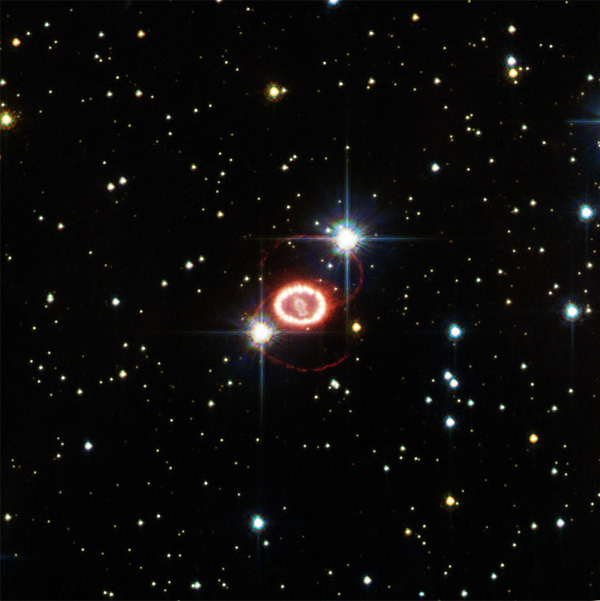
\includegraphics[width=0.6\textwidth]{../Images/SNe_1987a.jpg}
		            \caption{The shock wave from Supernova 1987a imaged by HST in 2006.\label{fig:SNe_1987a}}
		        \end{figure}
   			 % subsection supernovae_and_other_transient_sources (end)

		    \subsubsection*{Lower Redshift Sources and photometric scattering} % (fold)
		    \label{sub:lower_redshift_sources_and_photometric_scattering}
		        This category is likely to provide the greatest source of contamination for the surveyed area. It will do so increasingly at high redshifts where its affect on the faintest magnitudes is most greatly felt. Its affect is most influential with a small S/N ratio for the observations, by fixing this at a level of $S/N = 5$ we can be confident that the contamination will be low. Detecting a source in another band such as b435, v606, i775 for YJH photometry would class it as a contaminant and then should be removed from sample, however we wont use this as it would too greatly increase the time.
		    % subsection lower_redshift_sources_and_photometric_scattering (end)

    	% subsubsection sources_of_contamination (end)
    	\subsubsection{Eliminatiing Contaminants} % (fold)
    	\label{sub:eliminatiing_contaminants}
			The \emph{colour} of an object in photometry is defined as the difference in magnitude between two filters. If there are two filters, for example purposes let them be called A and B, where A has a lower central wavelength, the colour for an object in these two filters would be,
			\begin{align}
				m_A-m_B=-2.5\log\left(\frac{f_A}{f_B}\right).
			\end{align}
			This equation is specifically for the AB magnitude system and it is clear that if the colour is zero there is no change in flux for the object in those two filters. For other magnitude systems there would be a constant added to the right hand side of the equation as there is still a difference in flux between the two filters if the colour is zero. If the colour is positive it is said to be `red' and if it is negative it is said to be `blue', i.e. an aboject which is red between two filters has a lower flux in the blueward filter compared to the redward filter and an object which is red has a larger flux in the blueward filter than the redward one.  The larger the value is, it is said that the `redder' the object is. To eliminate candidates from observations, a colour-colour diagram can be made using three filters, with two colour values for each object. For instance if the observations were done in the J, H and K filters, the colour colour diagram would be (H-K) plotted against (J-H). Although this study does not take any observtions, colour diagrams can be built up for observations by simulating a catalog of lyman break galaxies at high redshift and determine colour windows for observations using the program Hyperz.
    	% subsection eliminatiing_contaminants (end)
	%subsection Eliminating_Contaminants (end)
% section contaminants (end)

    \subsection{Hyperz} %fold
	\label{sub:Hyperz}
		To eliminate contaminates and predict colour windows for observations the program Hyperz and its subprogram `make\_catalog' can be used to produce a catalog of synthetic galaxies and their magnitudes in different filters at different redshifts.

        \subsubsection{Inputs} %fold
        \label{subsub:Hyperz_inputs}
			The operation of the program is quite complex and is only summarised here. Also, the operation of make catalog is slightly different to Hyperz and a full manual for make catalog was not obtainable. The program starts with a sample Spectral Energy Distribution (SED) to  The Predictions group schecter function used the \SI{1500}{\angstrom} rest UV wavelength with the assumption that the flux from a lyman break galaxy was approximately the same for \SI{1350}{\angstrom} to \SI{1750}{\angstrom}. The program uses a known magnitude in a reference filter to convert to other bands. Using the Prediction's group program, a range of magnitudes can be found for a certain redshift interval by looking at the number of galaxies for a certain magnitude at a certain redshift. As the redshifted \SI{1500}{\angstrom} line will move with redshift, a range of reference filters were required to cover the redshift range for the observing strategy. As the flux is assumed to be constant over the range \SI{1350}{\angstrom}--\SI{1750}{\angstrom}, this meant a single filter could be used for a wide interval of redshifts. Below is a table listing the reference filters
		%subsubsection Inputs (end)

		\subsubsection{Reddening Law} % (fold)
		\label{ssub:reddening_law}
			\begin{align}
				f_\text{obs}(\lambda)=f_{int}(\lambda)10^{-0.4A_\lambda}
			\end{align}
			\begin{align}
				A_\lambda=k(\lambda)E(B-V)=\frac{k(\lambda)A_V}{R_V}
			\end{align}
			\begin{align}
				k(\lambda)=2.659(-1.857+\frac{1.040}{\lambda})+R_V for 0.63%{\mew}%m
			\end{align}

			To keep consistency between the two groups, the same cosmological constants were used as the predicitons group, which were: $\Omega_M=0.27$, $\Omega_\Lambda=0.73$ and $H_0=\SI{71}{\kilo\metre\per\second\per\mega\parsec}$.

			Conversions from Vega to AB are complex. Therefore conversions for a ground based telescope for typical filters have been used from \cite{???[Graham]} The only filter which wasn't comparable to another filter in \cite{???[Graham]} was the Y-filter for Euclid. As there was information for two filters either side of this filter, and noticing that the AB conversion increased with wavelength, an average value of the conversions for ... and ... to find a conversion for the Y band filter. The reference filters were from the database of filters that came with Hyperz and so came ready with conversions to AB. The conversions for the reference filters were applied for the input into the program, and the output magnitude in the various filters were changed to AB from Vega.
			\begin{table}[ht]
				\begin{center}
					\begin{tabular}{c|c}
						Filter band 	& M(AB)-M(Vega) \\
						\hline \hline
						I	& 0.5 \\
						Y 	& \\
						J 	& 0.9\\
						H 	& 1.4\\
						K 	& 1.9\\
					\end{tabular}
				\end{center}
				\caption{AB conversion}
				\label{tab:AB_conversion}
			\end{table}
			% subsubsection reddening_law (end)

			\subsubsection{Output} % (fold)
			\label{ssub:output}
				After running the executable file, the output is shown as in the example below for five galaxies,


				From the output, the colour of an object can be found from subtracting the magnitude of two filters, a colour diagram can then be plotted.

			% subsubsection output (end)
	%subsection Hyperz (end)

	\subsection{Results for Colour} %fold
	\label{sub:Results_for_Colour}
		Below are the results for four of the specified ranges, the redshift range 14 to 15 was not included here as there was an unresolved problem with the f275w filter on NIRcam, which will be discussed below.
		\begin{figure}[!htbp]
			\begin{minipage}[c]{0.5\linewidth}
				\centering
					\begingroup\endlinechar=-1
						\resizebox{\textwidth}{!}{%
							% GNUPLOT: LaTeX picture with Postscript
\begingroup
  \makeatletter
  \providecommand\color[2][]{%
    \GenericError{(gnuplot) \space\space\space\@spaces}{%
      Package color not loaded in conjunction with
      terminal option `colourtext'%
    }{See the gnuplot documentation for explanation.%
    }{Either use 'blacktext' in gnuplot or load the package
      color.sty in LaTeX.}%
    \renewcommand\color[2][]{}%
  }%
  \providecommand\includegraphics[2][]{%
    \GenericError{(gnuplot) \space\space\space\@spaces}{%
      Package graphicx or graphics not loaded%
    }{See the gnuplot documentation for explanation.%
    }{The gnuplot epslatex terminal needs graphicx.sty or graphics.sty.}%
    \renewcommand\includegraphics[2][]{}%
  }%
  \providecommand\rotatebox[2]{#2}%
  \@ifundefined{ifGPcolor}{%
    \newif\ifGPcolor
    \GPcolortrue
  }{}%
  \@ifundefined{ifGPblacktext}{%
    \newif\ifGPblacktext
    \GPblacktexttrue
  }{}%
  % define a \g@addto@macro without @ in the name:
  \let\gplgaddtomacro\g@addto@macro
  % define empty templates for all commands taking text:
  \gdef\gplbacktext{}%
  \gdef\gplfronttext{}%
  \makeatother
  \ifGPblacktext
    % no textcolor at all
    \def\colorrgb#1{}%
    \def\colorgray#1{}%
  \else
    % gray or color?
    \ifGPcolor
      \def\colorrgb#1{\color[rgb]{#1}}%
      \def\colorgray#1{\color[gray]{#1}}%
      \expandafter\def\csname LTw\endcsname{\color{white}}%
      \expandafter\def\csname LTb\endcsname{\color{black}}%
      \expandafter\def\csname LTa\endcsname{\color{black}}%
      \expandafter\def\csname LT0\endcsname{\color[rgb]{1,0,0}}%
      \expandafter\def\csname LT1\endcsname{\color[rgb]{0,1,0}}%
      \expandafter\def\csname LT2\endcsname{\color[rgb]{0,0,1}}%
      \expandafter\def\csname LT3\endcsname{\color[rgb]{1,0,1}}%
      \expandafter\def\csname LT4\endcsname{\color[rgb]{0,1,1}}%
      \expandafter\def\csname LT5\endcsname{\color[rgb]{1,1,0}}%
      \expandafter\def\csname LT6\endcsname{\color[rgb]{0,0,0}}%
      \expandafter\def\csname LT7\endcsname{\color[rgb]{1,0.3,0}}%
      \expandafter\def\csname LT8\endcsname{\color[rgb]{0.5,0.5,0.5}}%
    \else
      % gray
      \def\colorrgb#1{\color{black}}%
      \def\colorgray#1{\color[gray]{#1}}%
      \expandafter\def\csname LTw\endcsname{\color{white}}%
      \expandafter\def\csname LTb\endcsname{\color{black}}%
      \expandafter\def\csname LTa\endcsname{\color{black}}%
      \expandafter\def\csname LT0\endcsname{\color{black}}%
      \expandafter\def\csname LT1\endcsname{\color{black}}%
      \expandafter\def\csname LT2\endcsname{\color{black}}%
      \expandafter\def\csname LT3\endcsname{\color{black}}%
      \expandafter\def\csname LT4\endcsname{\color{black}}%
      \expandafter\def\csname LT5\endcsname{\color{black}}%
      \expandafter\def\csname LT6\endcsname{\color{black}}%
      \expandafter\def\csname LT7\endcsname{\color{black}}%
      \expandafter\def\csname LT8\endcsname{\color{black}}%
    \fi
  \fi
  \setlength{\unitlength}{0.0500bp}%
  \begin{picture}(7200.00,4320.00)%
    \gplgaddtomacro\gplbacktext{%
      \put(747,595){\makebox(0,0)[r]{\strut{} 3}}%
      \put(747,1047){\makebox(0,0)[r]{\strut{} 3.5}}%
      \put(747,1500){\makebox(0,0)[r]{\strut{} 4}}%
      \put(747,1952){\makebox(0,0)[r]{\strut{} 4.5}}%
      \put(747,2404){\makebox(0,0)[r]{\strut{} 5}}%
      \put(747,2856){\makebox(0,0)[r]{\strut{} 5.5}}%
      \put(747,3309){\makebox(0,0)[r]{\strut{} 6}}%
      \put(747,3761){\makebox(0,0)[r]{\strut{} 6.5}}%
      \put(849,409){\makebox(0,0){\strut{} 3.5}}%
      \put(1453,409){\makebox(0,0){\strut{} 4}}%
      \put(2058,409){\makebox(0,0){\strut{} 4.5}}%
      \put(2662,409){\makebox(0,0){\strut{} 5}}%
      \put(3267,409){\makebox(0,0){\strut{} 5.5}}%
      \put(3871,409){\makebox(0,0){\strut{} 6}}%
      \put(4475,409){\makebox(0,0){\strut{} 6.5}}%
      \put(5080,409){\makebox(0,0){\strut{} 7}}%
      \put(5684,409){\makebox(0,0){\strut{} 7.5}}%
      \put(6289,409){\makebox(0,0){\strut{} 8}}%
      \put(6893,409){\makebox(0,0){\strut{} 8.5}}%
      \csname LTb\endcsname%
      \put(144,2178){\rotatebox{-270}{\makebox(0,0){\strut{}f070w-f090w}}}%
      \csname LTb\endcsname%
      \put(3871,130){\makebox(0,0){\strut{}f090w-f115w}}%
      \put(3871,4040){\makebox(0,0){\strut{}Redshift 6--7.5}}%
    }%
    \gplgaddtomacro\gplfronttext{%
    }%
    \gplbacktext
    \put(0,0){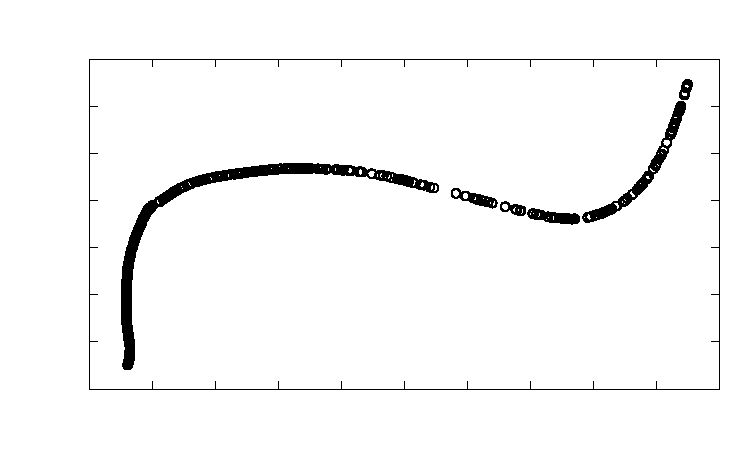
\includegraphics{GRAPH_color_graph1}}%
    \gplfronttext
  \end{picture}%
\endgroup

						}\endgroup
				\caption{A\label{fig:col1}}
			\end{minipage}
			\begin{minipage}[c]{0.5\linewidth}
				\centering
					\begingroup\endlinechar=-1
						\resizebox{\textwidth}{!}{%
							% GNUPLOT: LaTeX picture with Postscript
\begingroup
  \makeatletter
  \providecommand\color[2][]{%
    \GenericError{(gnuplot) \space\space\space\@spaces}{%
      Package color not loaded in conjunction with
      terminal option `colourtext'%
    }{See the gnuplot documentation for explanation.%
    }{Either use 'blacktext' in gnuplot or load the package
      color.sty in LaTeX.}%
    \renewcommand\color[2][]{}%
  }%
  \providecommand\includegraphics[2][]{%
    \GenericError{(gnuplot) \space\space\space\@spaces}{%
      Package graphicx or graphics not loaded%
    }{See the gnuplot documentation for explanation.%
    }{The gnuplot epslatex terminal needs graphicx.sty or graphics.sty.}%
    \renewcommand\includegraphics[2][]{}%
  }%
  \providecommand\rotatebox[2]{#2}%
  \@ifundefined{ifGPcolor}{%
    \newif\ifGPcolor
    \GPcolortrue
  }{}%
  \@ifundefined{ifGPblacktext}{%
    \newif\ifGPblacktext
    \GPblacktexttrue
  }{}%
  % define a \g@addto@macro without @ in the name:
  \let\gplgaddtomacro\g@addto@macro
  % define empty templates for all commands taking text:
  \gdef\gplbacktext{}%
  \gdef\gplfronttext{}%
  \makeatother
  \ifGPblacktext
    % no textcolor at all
    \def\colorrgb#1{}%
    \def\colorgray#1{}%
  \else
    % gray or color?
    \ifGPcolor
      \def\colorrgb#1{\color[rgb]{#1}}%
      \def\colorgray#1{\color[gray]{#1}}%
      \expandafter\def\csname LTw\endcsname{\color{white}}%
      \expandafter\def\csname LTb\endcsname{\color{black}}%
      \expandafter\def\csname LTa\endcsname{\color{black}}%
      \expandafter\def\csname LT0\endcsname{\color[rgb]{1,0,0}}%
      \expandafter\def\csname LT1\endcsname{\color[rgb]{0,1,0}}%
      \expandafter\def\csname LT2\endcsname{\color[rgb]{0,0,1}}%
      \expandafter\def\csname LT3\endcsname{\color[rgb]{1,0,1}}%
      \expandafter\def\csname LT4\endcsname{\color[rgb]{0,1,1}}%
      \expandafter\def\csname LT5\endcsname{\color[rgb]{1,1,0}}%
      \expandafter\def\csname LT6\endcsname{\color[rgb]{0,0,0}}%
      \expandafter\def\csname LT7\endcsname{\color[rgb]{1,0.3,0}}%
      \expandafter\def\csname LT8\endcsname{\color[rgb]{0.5,0.5,0.5}}%
    \else
      % gray
      \def\colorrgb#1{\color{black}}%
      \def\colorgray#1{\color[gray]{#1}}%
      \expandafter\def\csname LTw\endcsname{\color{white}}%
      \expandafter\def\csname LTb\endcsname{\color{black}}%
      \expandafter\def\csname LTa\endcsname{\color{black}}%
      \expandafter\def\csname LT0\endcsname{\color{black}}%
      \expandafter\def\csname LT1\endcsname{\color{black}}%
      \expandafter\def\csname LT2\endcsname{\color{black}}%
      \expandafter\def\csname LT3\endcsname{\color{black}}%
      \expandafter\def\csname LT4\endcsname{\color{black}}%
      \expandafter\def\csname LT5\endcsname{\color{black}}%
      \expandafter\def\csname LT6\endcsname{\color{black}}%
      \expandafter\def\csname LT7\endcsname{\color{black}}%
      \expandafter\def\csname LT8\endcsname{\color{black}}%
    \fi
  \fi
  \setlength{\unitlength}{0.0500bp}%
  \begin{picture}(7200.00,4320.00)%
    \gplgaddtomacro\gplbacktext{%
      \put(849,595){\makebox(0,0)[r]{\strut{} 8}}%
      \put(849,991){\makebox(0,0)[r]{\strut{} 8.5}}%
      \put(849,1387){\makebox(0,0)[r]{\strut{} 9}}%
      \put(849,1782){\makebox(0,0)[r]{\strut{} 9.5}}%
      \put(849,2178){\makebox(0,0)[r]{\strut{} 10}}%
      \put(849,2574){\makebox(0,0)[r]{\strut{} 10.5}}%
      \put(849,2970){\makebox(0,0)[r]{\strut{} 11}}%
      \put(849,3365){\makebox(0,0)[r]{\strut{} 11.5}}%
      \put(849,3761){\makebox(0,0)[r]{\strut{} 12}}%
      \put(951,409){\makebox(0,0){\strut{} 2.5}}%
      \put(1694,409){\makebox(0,0){\strut{} 2.55}}%
      \put(2436,409){\makebox(0,0){\strut{} 2.6}}%
      \put(3179,409){\makebox(0,0){\strut{} 2.65}}%
      \put(3922,409){\makebox(0,0){\strut{} 2.7}}%
      \put(4665,409){\makebox(0,0){\strut{} 2.75}}%
      \put(5407,409){\makebox(0,0){\strut{} 2.8}}%
      \put(6150,409){\makebox(0,0){\strut{} 2.85}}%
      \put(6893,409){\makebox(0,0){\strut{} 2.9}}%
      \csname LTb\endcsname%
      \put(144,2178){\rotatebox{-270}{\makebox(0,0){\strut{}f070w-f090w}}}%
      \csname LTb\endcsname%
      \put(3922,130){\makebox(0,0){\strut{}f090w-f115w}}%
      \put(3922,4040){\makebox(0,0){\strut{}Redshift 7.5--8.5}}%
    }%
    \gplgaddtomacro\gplfronttext{%
    }%
    \gplbacktext
    \put(0,0){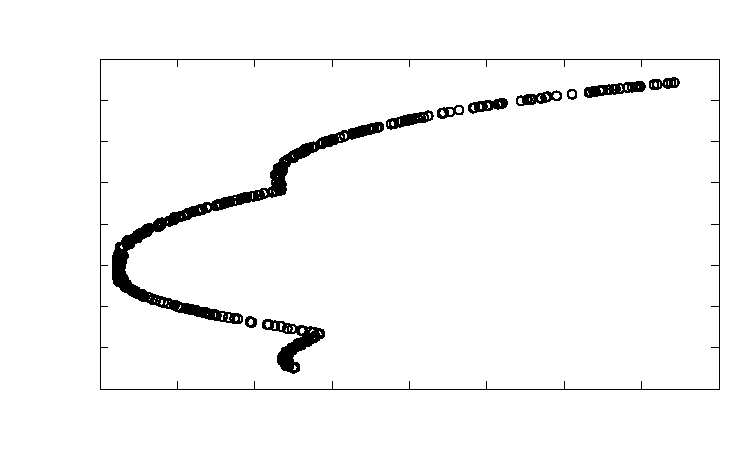
\includegraphics{GRAPH_color_graph2}}%
    \gplfronttext
  \end{picture}%
\endgroup

						}\endgroup
				\caption{B\label{fig:col2}}
			\end{minipage}
			\begin{minipage}[c]{0.5\linewidth}
				\centering
					\begingroup\endlinechar=-1
						\resizebox{\textwidth}{!}{%
							% GNUPLOT: LaTeX picture with Postscript
\begingroup
  \makeatletter
  \providecommand\color[2][]{%
    \GenericError{(gnuplot) \space\space\space\@spaces}{%
      Package color not loaded in conjunction with
      terminal option `colourtext'%
    }{See the gnuplot documentation for explanation.%
    }{Either use 'blacktext' in gnuplot or load the package
      color.sty in LaTeX.}%
    \renewcommand\color[2][]{}%
  }%
  \providecommand\includegraphics[2][]{%
    \GenericError{(gnuplot) \space\space\space\@spaces}{%
      Package graphicx or graphics not loaded%
    }{See the gnuplot documentation for explanation.%
    }{The gnuplot epslatex terminal needs graphicx.sty or graphics.sty.}%
    \renewcommand\includegraphics[2][]{}%
  }%
  \providecommand\rotatebox[2]{#2}%
  \@ifundefined{ifGPcolor}{%
    \newif\ifGPcolor
    \GPcolortrue
  }{}%
  \@ifundefined{ifGPblacktext}{%
    \newif\ifGPblacktext
    \GPblacktexttrue
  }{}%
  % define a \g@addto@macro without @ in the name:
  \let\gplgaddtomacro\g@addto@macro
  % define empty templates for all commands taking text:
  \gdef\gplbacktext{}%
  \gdef\gplfronttext{}%
  \makeatother
  \ifGPblacktext
    % no textcolor at all
    \def\colorrgb#1{}%
    \def\colorgray#1{}%
  \else
    % gray or color?
    \ifGPcolor
      \def\colorrgb#1{\color[rgb]{#1}}%
      \def\colorgray#1{\color[gray]{#1}}%
      \expandafter\def\csname LTw\endcsname{\color{white}}%
      \expandafter\def\csname LTb\endcsname{\color{black}}%
      \expandafter\def\csname LTa\endcsname{\color{black}}%
      \expandafter\def\csname LT0\endcsname{\color[rgb]{1,0,0}}%
      \expandafter\def\csname LT1\endcsname{\color[rgb]{0,1,0}}%
      \expandafter\def\csname LT2\endcsname{\color[rgb]{0,0,1}}%
      \expandafter\def\csname LT3\endcsname{\color[rgb]{1,0,1}}%
      \expandafter\def\csname LT4\endcsname{\color[rgb]{0,1,1}}%
      \expandafter\def\csname LT5\endcsname{\color[rgb]{1,1,0}}%
      \expandafter\def\csname LT6\endcsname{\color[rgb]{0,0,0}}%
      \expandafter\def\csname LT7\endcsname{\color[rgb]{1,0.3,0}}%
      \expandafter\def\csname LT8\endcsname{\color[rgb]{0.5,0.5,0.5}}%
    \else
      % gray
      \def\colorrgb#1{\color{black}}%
      \def\colorgray#1{\color[gray]{#1}}%
      \expandafter\def\csname LTw\endcsname{\color{white}}%
      \expandafter\def\csname LTb\endcsname{\color{black}}%
      \expandafter\def\csname LTa\endcsname{\color{black}}%
      \expandafter\def\csname LT0\endcsname{\color{black}}%
      \expandafter\def\csname LT1\endcsname{\color{black}}%
      \expandafter\def\csname LT2\endcsname{\color{black}}%
      \expandafter\def\csname LT3\endcsname{\color{black}}%
      \expandafter\def\csname LT4\endcsname{\color{black}}%
      \expandafter\def\csname LT5\endcsname{\color{black}}%
      \expandafter\def\csname LT6\endcsname{\color{black}}%
      \expandafter\def\csname LT7\endcsname{\color{black}}%
      \expandafter\def\csname LT8\endcsname{\color{black}}%
    \fi
  \fi
  \setlength{\unitlength}{0.0500bp}%
  \begin{picture}(7200.00,4320.00)%
    \gplgaddtomacro\gplbacktext{%
      \put(849,595){\makebox(0,0)[r]{\strut{} 11}}%
      \put(849,912){\makebox(0,0)[r]{\strut{} 11.5}}%
      \put(849,1228){\makebox(0,0)[r]{\strut{} 12}}%
      \put(849,1545){\makebox(0,0)[r]{\strut{} 12.5}}%
      \put(849,1861){\makebox(0,0)[r]{\strut{} 13}}%
      \put(849,2178){\makebox(0,0)[r]{\strut{} 13.5}}%
      \put(849,2495){\makebox(0,0)[r]{\strut{} 14}}%
      \put(849,2811){\makebox(0,0)[r]{\strut{} 14.5}}%
      \put(849,3128){\makebox(0,0)[r]{\strut{} 15}}%
      \put(849,3444){\makebox(0,0)[r]{\strut{} 15.5}}%
      \put(849,3761){\makebox(0,0)[r]{\strut{} 16}}%
      \put(951,409){\makebox(0,0){\strut{} 1.5}}%
      \put(1694,409){\makebox(0,0){\strut{} 2}}%
      \put(2437,409){\makebox(0,0){\strut{} 2.5}}%
      \put(3179,409){\makebox(0,0){\strut{} 3}}%
      \put(3922,409){\makebox(0,0){\strut{} 3.5}}%
      \put(4665,409){\makebox(0,0){\strut{} 4}}%
      \put(5408,409){\makebox(0,0){\strut{} 4.5}}%
      \put(6150,409){\makebox(0,0){\strut{} 5}}%
      \put(6893,409){\makebox(0,0){\strut{} 5.5}}%
      \csname LTb\endcsname%
      \put(144,2178){\rotatebox{-270}{\makebox(0,0){\strut{}Y-J}}}%
      \csname LTb\endcsname%
      \put(3922,130){\makebox(0,0){\strut{}J-H}}%
      \put(3922,4040){\makebox(0,0){\strut{}Redshift 8.5--10.1}}%
    }%
    \gplgaddtomacro\gplfronttext{%
    }%
    \gplbacktext
    \put(0,0){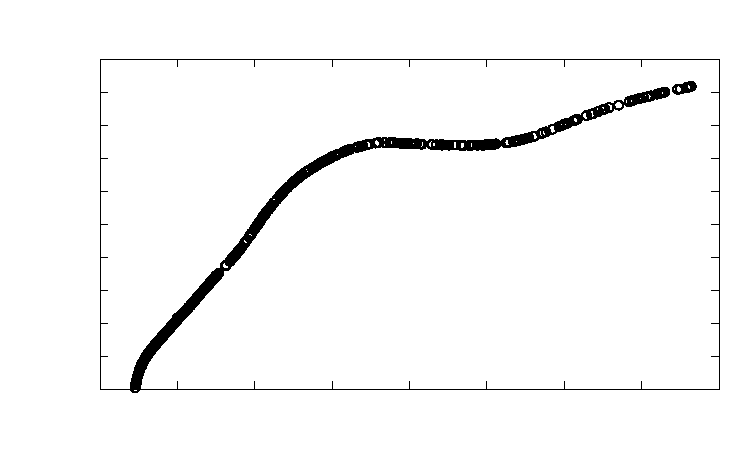
\includegraphics{GRAPH_color_graph3}}%
    \gplfronttext
  \end{picture}%
\endgroup

						}\endgroup
				\caption{C\label{fig:col3}}
			\end{minipage}
			\begin{minipage}[c]{0.5\linewidth}
				\centering
					\begingroup\endlinechar=-1
						\resizebox{\textwidth}{!}{%
							% GNUPLOT: LaTeX picture with Postscript
\begingroup
  \makeatletter
  \providecommand\color[2][]{%
    \GenericError{(gnuplot) \space\space\space\@spaces}{%
      Package color not loaded in conjunction with
      terminal option `colourtext'%
    }{See the gnuplot documentation for explanation.%
    }{Either use 'blacktext' in gnuplot or load the package
      color.sty in LaTeX.}%
    \renewcommand\color[2][]{}%
  }%
  \providecommand\includegraphics[2][]{%
    \GenericError{(gnuplot) \space\space\space\@spaces}{%
      Package graphicx or graphics not loaded%
    }{See the gnuplot documentation for explanation.%
    }{The gnuplot epslatex terminal needs graphicx.sty or graphics.sty.}%
    \renewcommand\includegraphics[2][]{}%
  }%
  \providecommand\rotatebox[2]{#2}%
  \@ifundefined{ifGPcolor}{%
    \newif\ifGPcolor
    \GPcolortrue
  }{}%
  \@ifundefined{ifGPblacktext}{%
    \newif\ifGPblacktext
    \GPblacktexttrue
  }{}%
  % define a \g@addto@macro without @ in the name:
  \let\gplgaddtomacro\g@addto@macro
  % define empty templates for all commands taking text:
  \gdef\gplbacktext{}%
  \gdef\gplfronttext{}%
  \makeatother
  \ifGPblacktext
    % no textcolor at all
    \def\colorrgb#1{}%
    \def\colorgray#1{}%
  \else
    % gray or color?
    \ifGPcolor
      \def\colorrgb#1{\color[rgb]{#1}}%
      \def\colorgray#1{\color[gray]{#1}}%
      \expandafter\def\csname LTw\endcsname{\color{white}}%
      \expandafter\def\csname LTb\endcsname{\color{black}}%
      \expandafter\def\csname LTa\endcsname{\color{black}}%
      \expandafter\def\csname LT0\endcsname{\color[rgb]{1,0,0}}%
      \expandafter\def\csname LT1\endcsname{\color[rgb]{0,1,0}}%
      \expandafter\def\csname LT2\endcsname{\color[rgb]{0,0,1}}%
      \expandafter\def\csname LT3\endcsname{\color[rgb]{1,0,1}}%
      \expandafter\def\csname LT4\endcsname{\color[rgb]{0,1,1}}%
      \expandafter\def\csname LT5\endcsname{\color[rgb]{1,1,0}}%
      \expandafter\def\csname LT6\endcsname{\color[rgb]{0,0,0}}%
      \expandafter\def\csname LT7\endcsname{\color[rgb]{1,0.3,0}}%
      \expandafter\def\csname LT8\endcsname{\color[rgb]{0.5,0.5,0.5}}%
    \else
      % gray
      \def\colorrgb#1{\color{black}}%
      \def\colorgray#1{\color[gray]{#1}}%
      \expandafter\def\csname LTw\endcsname{\color{white}}%
      \expandafter\def\csname LTb\endcsname{\color{black}}%
      \expandafter\def\csname LTa\endcsname{\color{black}}%
      \expandafter\def\csname LT0\endcsname{\color{black}}%
      \expandafter\def\csname LT1\endcsname{\color{black}}%
      \expandafter\def\csname LT2\endcsname{\color{black}}%
      \expandafter\def\csname LT3\endcsname{\color{black}}%
      \expandafter\def\csname LT4\endcsname{\color{black}}%
      \expandafter\def\csname LT5\endcsname{\color{black}}%
      \expandafter\def\csname LT6\endcsname{\color{black}}%
      \expandafter\def\csname LT7\endcsname{\color{black}}%
      \expandafter\def\csname LT8\endcsname{\color{black}}%
    \fi
  \fi
  \setlength{\unitlength}{0.0500bp}%
  \begin{picture}(7200.00,4320.00)%
    \gplgaddtomacro\gplbacktext{%
      \put(645,595){\makebox(0,0)[r]{\strut{} 10}}%
      \put(645,947){\makebox(0,0)[r]{\strut{} 15}}%
      \put(645,1299){\makebox(0,0)[r]{\strut{} 20}}%
      \put(645,1650){\makebox(0,0)[r]{\strut{} 25}}%
      \put(645,2002){\makebox(0,0)[r]{\strut{} 30}}%
      \put(645,2354){\makebox(0,0)[r]{\strut{} 35}}%
      \put(645,2706){\makebox(0,0)[r]{\strut{} 40}}%
      \put(645,3057){\makebox(0,0)[r]{\strut{} 45}}%
      \put(645,3409){\makebox(0,0)[r]{\strut{} 50}}%
      \put(645,3761){\makebox(0,0)[r]{\strut{} 55}}%
      \put(747,409){\makebox(0,0){\strut{} 0}}%
      \put(1515,409){\makebox(0,0){\strut{} 2}}%
      \put(2284,409){\makebox(0,0){\strut{} 4}}%
      \put(3052,409){\makebox(0,0){\strut{} 6}}%
      \put(3820,409){\makebox(0,0){\strut{} 8}}%
      \put(4588,409){\makebox(0,0){\strut{} 10}}%
      \put(5357,409){\makebox(0,0){\strut{} 12}}%
      \put(6125,409){\makebox(0,0){\strut{} 14}}%
      \put(6893,409){\makebox(0,0){\strut{} 16}}%
      \csname LTb\endcsname%
      \put(144,2178){\rotatebox{-270}{\makebox(0,0){\strut{}f150w-f200w}}}%
      \csname LTb\endcsname%
      \put(3820,130){\makebox(0,0){\strut{}f115w-f150w}}%
      \put(3820,4040){\makebox(0,0){\strut{}Redshift 10--14}}%
    }%
    \gplgaddtomacro\gplfronttext{%
    }%
    \gplbacktext
    \put(0,0){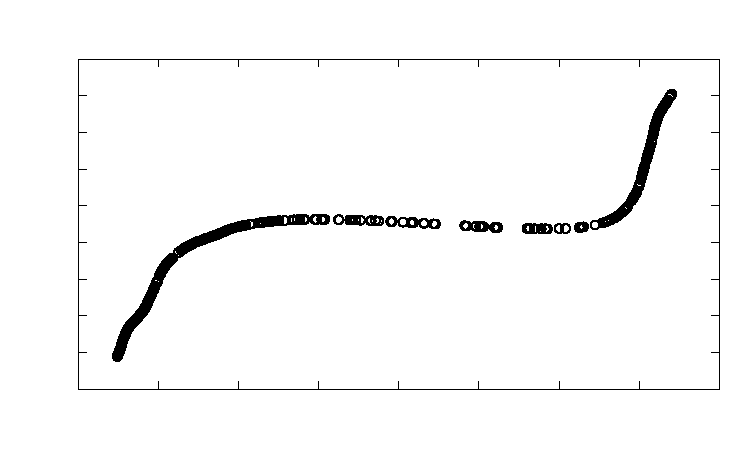
\includegraphics{GRAPH_color_graph4}}%
    \gplfronttext
  \end{picture}%
\endgroup

						}\endgroup
				\caption{D\label{fig:col4}}
			\end{minipage}
			\caption{Graphs showing the colour-colour regions for \\
			(A) z=6-7.5. The colour window was defined as $f070w-f090w{\ge}3.257$ and $f090w-f115w{\le}8.242$,\\
			(B) z=7.5-8.5. The colour window was defined as $f090w-f115w{\ge}8.251$ and $f115w-f150w{\le}2.869$, \\
			(C) z=8.54-10.1. The colour window was defined as $Y-J{\ge}11.019$ and $J-H{\le}5.298$, \\
			(D) z=10-14. The colour window was defined as $f115w-f150w{\ge}14.439$ and $f150w-f200w{\le}14.815$}
		\end{figure}

		% \begin{figure}[!htbp]
		% 	\centering
		% 		\begingroup\endlinechar=-1
		% 			\resizebox{0.7\textwidth}{!}{%
		% 				% GNUPLOT: LaTeX picture with Postscript
\begingroup
  \makeatletter
  \providecommand\color[2][]{%
    \GenericError{(gnuplot) \space\space\space\@spaces}{%
      Package color not loaded in conjunction with
      terminal option `colourtext'%
    }{See the gnuplot documentation for explanation.%
    }{Either use 'blacktext' in gnuplot or load the package
      color.sty in LaTeX.}%
    \renewcommand\color[2][]{}%
  }%
  \providecommand\includegraphics[2][]{%
    \GenericError{(gnuplot) \space\space\space\@spaces}{%
      Package graphicx or graphics not loaded%
    }{See the gnuplot documentation for explanation.%
    }{The gnuplot epslatex terminal needs graphicx.sty or graphics.sty.}%
    \renewcommand\includegraphics[2][]{}%
  }%
  \providecommand\rotatebox[2]{#2}%
  \@ifundefined{ifGPcolor}{%
    \newif\ifGPcolor
    \GPcolortrue
  }{}%
  \@ifundefined{ifGPblacktext}{%
    \newif\ifGPblacktext
    \GPblacktexttrue
  }{}%
  % define a \g@addto@macro without @ in the name:
  \let\gplgaddtomacro\g@addto@macro
  % define empty templates for all commands taking text:
  \gdef\gplbacktext{}%
  \gdef\gplfronttext{}%
  \makeatother
  \ifGPblacktext
    % no textcolor at all
    \def\colorrgb#1{}%
    \def\colorgray#1{}%
  \else
    % gray or color?
    \ifGPcolor
      \def\colorrgb#1{\color[rgb]{#1}}%
      \def\colorgray#1{\color[gray]{#1}}%
      \expandafter\def\csname LTw\endcsname{\color{white}}%
      \expandafter\def\csname LTb\endcsname{\color{black}}%
      \expandafter\def\csname LTa\endcsname{\color{black}}%
      \expandafter\def\csname LT0\endcsname{\color[rgb]{1,0,0}}%
      \expandafter\def\csname LT1\endcsname{\color[rgb]{0,1,0}}%
      \expandafter\def\csname LT2\endcsname{\color[rgb]{0,0,1}}%
      \expandafter\def\csname LT3\endcsname{\color[rgb]{1,0,1}}%
      \expandafter\def\csname LT4\endcsname{\color[rgb]{0,1,1}}%
      \expandafter\def\csname LT5\endcsname{\color[rgb]{1,1,0}}%
      \expandafter\def\csname LT6\endcsname{\color[rgb]{0,0,0}}%
      \expandafter\def\csname LT7\endcsname{\color[rgb]{1,0.3,0}}%
      \expandafter\def\csname LT8\endcsname{\color[rgb]{0.5,0.5,0.5}}%
    \else
      % gray
      \def\colorrgb#1{\color{black}}%
      \def\colorgray#1{\color[gray]{#1}}%
      \expandafter\def\csname LTw\endcsname{\color{white}}%
      \expandafter\def\csname LTb\endcsname{\color{black}}%
      \expandafter\def\csname LTa\endcsname{\color{black}}%
      \expandafter\def\csname LT0\endcsname{\color{black}}%
      \expandafter\def\csname LT1\endcsname{\color{black}}%
      \expandafter\def\csname LT2\endcsname{\color{black}}%
      \expandafter\def\csname LT3\endcsname{\color{black}}%
      \expandafter\def\csname LT4\endcsname{\color{black}}%
      \expandafter\def\csname LT5\endcsname{\color{black}}%
      \expandafter\def\csname LT6\endcsname{\color{black}}%
      \expandafter\def\csname LT7\endcsname{\color{black}}%
      \expandafter\def\csname LT8\endcsname{\color{black}}%
    \fi
  \fi
  \setlength{\unitlength}{0.0500bp}%
  \begin{picture}(7200.00,4320.00)%
    \gplgaddtomacro\gplbacktext{%
      \put(747,595){\makebox(0,0)[r]{\strut{} 3}}%
      \put(747,1047){\makebox(0,0)[r]{\strut{} 3.5}}%
      \put(747,1500){\makebox(0,0)[r]{\strut{} 4}}%
      \put(747,1952){\makebox(0,0)[r]{\strut{} 4.5}}%
      \put(747,2404){\makebox(0,0)[r]{\strut{} 5}}%
      \put(747,2856){\makebox(0,0)[r]{\strut{} 5.5}}%
      \put(747,3309){\makebox(0,0)[r]{\strut{} 6}}%
      \put(747,3761){\makebox(0,0)[r]{\strut{} 6.5}}%
      \put(849,409){\makebox(0,0){\strut{} 3.5}}%
      \put(1453,409){\makebox(0,0){\strut{} 4}}%
      \put(2058,409){\makebox(0,0){\strut{} 4.5}}%
      \put(2662,409){\makebox(0,0){\strut{} 5}}%
      \put(3267,409){\makebox(0,0){\strut{} 5.5}}%
      \put(3871,409){\makebox(0,0){\strut{} 6}}%
      \put(4475,409){\makebox(0,0){\strut{} 6.5}}%
      \put(5080,409){\makebox(0,0){\strut{} 7}}%
      \put(5684,409){\makebox(0,0){\strut{} 7.5}}%
      \put(6289,409){\makebox(0,0){\strut{} 8}}%
      \put(6893,409){\makebox(0,0){\strut{} 8.5}}%
      \csname LTb\endcsname%
      \put(144,2178){\rotatebox{-270}{\makebox(0,0){\strut{}f070w-f090w}}}%
      \csname LTb\endcsname%
      \put(3871,130){\makebox(0,0){\strut{}f090w-f115w}}%
      \put(3871,4040){\makebox(0,0){\strut{}Redshift 6--7.5}}%
    }%
    \gplgaddtomacro\gplfronttext{%
    }%
    \gplbacktext
    \put(0,0){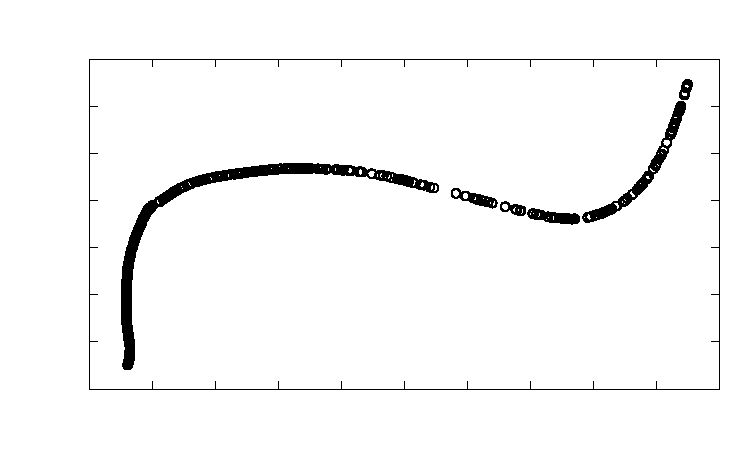
\includegraphics{GRAPH_color_graph1}}%
    \gplfronttext
  \end{picture}%
\endgroup

		% 			}\endgroup
		% 	\caption{Graph showing the colour-colour region for z=6-7.5. The colour window was defined as $f070w-f090w{\ge}3.257$ and $f090w-f115w{\le}8.242$.\label{fig:col1}}
		% \end{figure}
		% \begin{figure}[!htbp]
		% 	\centering
		% 		\begingroup\endlinechar=-1
		% 			\resizebox{0.7\textwidth}{!}{%
		% 				% GNUPLOT: LaTeX picture with Postscript
\begingroup
  \makeatletter
  \providecommand\color[2][]{%
    \GenericError{(gnuplot) \space\space\space\@spaces}{%
      Package color not loaded in conjunction with
      terminal option `colourtext'%
    }{See the gnuplot documentation for explanation.%
    }{Either use 'blacktext' in gnuplot or load the package
      color.sty in LaTeX.}%
    \renewcommand\color[2][]{}%
  }%
  \providecommand\includegraphics[2][]{%
    \GenericError{(gnuplot) \space\space\space\@spaces}{%
      Package graphicx or graphics not loaded%
    }{See the gnuplot documentation for explanation.%
    }{The gnuplot epslatex terminal needs graphicx.sty or graphics.sty.}%
    \renewcommand\includegraphics[2][]{}%
  }%
  \providecommand\rotatebox[2]{#2}%
  \@ifundefined{ifGPcolor}{%
    \newif\ifGPcolor
    \GPcolortrue
  }{}%
  \@ifundefined{ifGPblacktext}{%
    \newif\ifGPblacktext
    \GPblacktexttrue
  }{}%
  % define a \g@addto@macro without @ in the name:
  \let\gplgaddtomacro\g@addto@macro
  % define empty templates for all commands taking text:
  \gdef\gplbacktext{}%
  \gdef\gplfronttext{}%
  \makeatother
  \ifGPblacktext
    % no textcolor at all
    \def\colorrgb#1{}%
    \def\colorgray#1{}%
  \else
    % gray or color?
    \ifGPcolor
      \def\colorrgb#1{\color[rgb]{#1}}%
      \def\colorgray#1{\color[gray]{#1}}%
      \expandafter\def\csname LTw\endcsname{\color{white}}%
      \expandafter\def\csname LTb\endcsname{\color{black}}%
      \expandafter\def\csname LTa\endcsname{\color{black}}%
      \expandafter\def\csname LT0\endcsname{\color[rgb]{1,0,0}}%
      \expandafter\def\csname LT1\endcsname{\color[rgb]{0,1,0}}%
      \expandafter\def\csname LT2\endcsname{\color[rgb]{0,0,1}}%
      \expandafter\def\csname LT3\endcsname{\color[rgb]{1,0,1}}%
      \expandafter\def\csname LT4\endcsname{\color[rgb]{0,1,1}}%
      \expandafter\def\csname LT5\endcsname{\color[rgb]{1,1,0}}%
      \expandafter\def\csname LT6\endcsname{\color[rgb]{0,0,0}}%
      \expandafter\def\csname LT7\endcsname{\color[rgb]{1,0.3,0}}%
      \expandafter\def\csname LT8\endcsname{\color[rgb]{0.5,0.5,0.5}}%
    \else
      % gray
      \def\colorrgb#1{\color{black}}%
      \def\colorgray#1{\color[gray]{#1}}%
      \expandafter\def\csname LTw\endcsname{\color{white}}%
      \expandafter\def\csname LTb\endcsname{\color{black}}%
      \expandafter\def\csname LTa\endcsname{\color{black}}%
      \expandafter\def\csname LT0\endcsname{\color{black}}%
      \expandafter\def\csname LT1\endcsname{\color{black}}%
      \expandafter\def\csname LT2\endcsname{\color{black}}%
      \expandafter\def\csname LT3\endcsname{\color{black}}%
      \expandafter\def\csname LT4\endcsname{\color{black}}%
      \expandafter\def\csname LT5\endcsname{\color{black}}%
      \expandafter\def\csname LT6\endcsname{\color{black}}%
      \expandafter\def\csname LT7\endcsname{\color{black}}%
      \expandafter\def\csname LT8\endcsname{\color{black}}%
    \fi
  \fi
  \setlength{\unitlength}{0.0500bp}%
  \begin{picture}(7200.00,4320.00)%
    \gplgaddtomacro\gplbacktext{%
      \put(849,595){\makebox(0,0)[r]{\strut{} 8}}%
      \put(849,991){\makebox(0,0)[r]{\strut{} 8.5}}%
      \put(849,1387){\makebox(0,0)[r]{\strut{} 9}}%
      \put(849,1782){\makebox(0,0)[r]{\strut{} 9.5}}%
      \put(849,2178){\makebox(0,0)[r]{\strut{} 10}}%
      \put(849,2574){\makebox(0,0)[r]{\strut{} 10.5}}%
      \put(849,2970){\makebox(0,0)[r]{\strut{} 11}}%
      \put(849,3365){\makebox(0,0)[r]{\strut{} 11.5}}%
      \put(849,3761){\makebox(0,0)[r]{\strut{} 12}}%
      \put(951,409){\makebox(0,0){\strut{} 2.5}}%
      \put(1694,409){\makebox(0,0){\strut{} 2.55}}%
      \put(2436,409){\makebox(0,0){\strut{} 2.6}}%
      \put(3179,409){\makebox(0,0){\strut{} 2.65}}%
      \put(3922,409){\makebox(0,0){\strut{} 2.7}}%
      \put(4665,409){\makebox(0,0){\strut{} 2.75}}%
      \put(5407,409){\makebox(0,0){\strut{} 2.8}}%
      \put(6150,409){\makebox(0,0){\strut{} 2.85}}%
      \put(6893,409){\makebox(0,0){\strut{} 2.9}}%
      \csname LTb\endcsname%
      \put(144,2178){\rotatebox{-270}{\makebox(0,0){\strut{}f070w-f090w}}}%
      \csname LTb\endcsname%
      \put(3922,130){\makebox(0,0){\strut{}f090w-f115w}}%
      \put(3922,4040){\makebox(0,0){\strut{}Redshift 7.5--8.5}}%
    }%
    \gplgaddtomacro\gplfronttext{%
    }%
    \gplbacktext
    \put(0,0){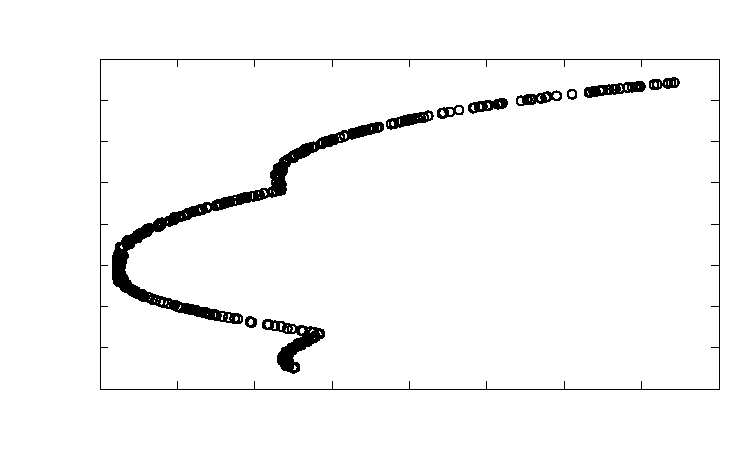
\includegraphics{GRAPH_color_graph2}}%
    \gplfronttext
  \end{picture}%
\endgroup

		% 			}\endgroup
		% 	\caption{Graph showing the colour-colour region for z=7.5-8.5. The colour window was defined as $f090w-f115w{\ge}8.251$ and $f115w-f150w{\le}2.869$\label{fig:col2}}
		% \end{figure}
		% \begin{figure}[!htbp]
		% 	\centering
		% 		\begingroup\endlinechar=-1
		% 			\resizebox{0.7\textwidth}{!}{%
		% 				% GNUPLOT: LaTeX picture with Postscript
\begingroup
  \makeatletter
  \providecommand\color[2][]{%
    \GenericError{(gnuplot) \space\space\space\@spaces}{%
      Package color not loaded in conjunction with
      terminal option `colourtext'%
    }{See the gnuplot documentation for explanation.%
    }{Either use 'blacktext' in gnuplot or load the package
      color.sty in LaTeX.}%
    \renewcommand\color[2][]{}%
  }%
  \providecommand\includegraphics[2][]{%
    \GenericError{(gnuplot) \space\space\space\@spaces}{%
      Package graphicx or graphics not loaded%
    }{See the gnuplot documentation for explanation.%
    }{The gnuplot epslatex terminal needs graphicx.sty or graphics.sty.}%
    \renewcommand\includegraphics[2][]{}%
  }%
  \providecommand\rotatebox[2]{#2}%
  \@ifundefined{ifGPcolor}{%
    \newif\ifGPcolor
    \GPcolortrue
  }{}%
  \@ifundefined{ifGPblacktext}{%
    \newif\ifGPblacktext
    \GPblacktexttrue
  }{}%
  % define a \g@addto@macro without @ in the name:
  \let\gplgaddtomacro\g@addto@macro
  % define empty templates for all commands taking text:
  \gdef\gplbacktext{}%
  \gdef\gplfronttext{}%
  \makeatother
  \ifGPblacktext
    % no textcolor at all
    \def\colorrgb#1{}%
    \def\colorgray#1{}%
  \else
    % gray or color?
    \ifGPcolor
      \def\colorrgb#1{\color[rgb]{#1}}%
      \def\colorgray#1{\color[gray]{#1}}%
      \expandafter\def\csname LTw\endcsname{\color{white}}%
      \expandafter\def\csname LTb\endcsname{\color{black}}%
      \expandafter\def\csname LTa\endcsname{\color{black}}%
      \expandafter\def\csname LT0\endcsname{\color[rgb]{1,0,0}}%
      \expandafter\def\csname LT1\endcsname{\color[rgb]{0,1,0}}%
      \expandafter\def\csname LT2\endcsname{\color[rgb]{0,0,1}}%
      \expandafter\def\csname LT3\endcsname{\color[rgb]{1,0,1}}%
      \expandafter\def\csname LT4\endcsname{\color[rgb]{0,1,1}}%
      \expandafter\def\csname LT5\endcsname{\color[rgb]{1,1,0}}%
      \expandafter\def\csname LT6\endcsname{\color[rgb]{0,0,0}}%
      \expandafter\def\csname LT7\endcsname{\color[rgb]{1,0.3,0}}%
      \expandafter\def\csname LT8\endcsname{\color[rgb]{0.5,0.5,0.5}}%
    \else
      % gray
      \def\colorrgb#1{\color{black}}%
      \def\colorgray#1{\color[gray]{#1}}%
      \expandafter\def\csname LTw\endcsname{\color{white}}%
      \expandafter\def\csname LTb\endcsname{\color{black}}%
      \expandafter\def\csname LTa\endcsname{\color{black}}%
      \expandafter\def\csname LT0\endcsname{\color{black}}%
      \expandafter\def\csname LT1\endcsname{\color{black}}%
      \expandafter\def\csname LT2\endcsname{\color{black}}%
      \expandafter\def\csname LT3\endcsname{\color{black}}%
      \expandafter\def\csname LT4\endcsname{\color{black}}%
      \expandafter\def\csname LT5\endcsname{\color{black}}%
      \expandafter\def\csname LT6\endcsname{\color{black}}%
      \expandafter\def\csname LT7\endcsname{\color{black}}%
      \expandafter\def\csname LT8\endcsname{\color{black}}%
    \fi
  \fi
  \setlength{\unitlength}{0.0500bp}%
  \begin{picture}(7200.00,4320.00)%
    \gplgaddtomacro\gplbacktext{%
      \put(849,595){\makebox(0,0)[r]{\strut{} 11}}%
      \put(849,912){\makebox(0,0)[r]{\strut{} 11.5}}%
      \put(849,1228){\makebox(0,0)[r]{\strut{} 12}}%
      \put(849,1545){\makebox(0,0)[r]{\strut{} 12.5}}%
      \put(849,1861){\makebox(0,0)[r]{\strut{} 13}}%
      \put(849,2178){\makebox(0,0)[r]{\strut{} 13.5}}%
      \put(849,2495){\makebox(0,0)[r]{\strut{} 14}}%
      \put(849,2811){\makebox(0,0)[r]{\strut{} 14.5}}%
      \put(849,3128){\makebox(0,0)[r]{\strut{} 15}}%
      \put(849,3444){\makebox(0,0)[r]{\strut{} 15.5}}%
      \put(849,3761){\makebox(0,0)[r]{\strut{} 16}}%
      \put(951,409){\makebox(0,0){\strut{} 1.5}}%
      \put(1694,409){\makebox(0,0){\strut{} 2}}%
      \put(2437,409){\makebox(0,0){\strut{} 2.5}}%
      \put(3179,409){\makebox(0,0){\strut{} 3}}%
      \put(3922,409){\makebox(0,0){\strut{} 3.5}}%
      \put(4665,409){\makebox(0,0){\strut{} 4}}%
      \put(5408,409){\makebox(0,0){\strut{} 4.5}}%
      \put(6150,409){\makebox(0,0){\strut{} 5}}%
      \put(6893,409){\makebox(0,0){\strut{} 5.5}}%
      \csname LTb\endcsname%
      \put(144,2178){\rotatebox{-270}{\makebox(0,0){\strut{}Y-J}}}%
      \csname LTb\endcsname%
      \put(3922,130){\makebox(0,0){\strut{}J-H}}%
      \put(3922,4040){\makebox(0,0){\strut{}Redshift 8.5--10.1}}%
    }%
    \gplgaddtomacro\gplfronttext{%
    }%
    \gplbacktext
    \put(0,0){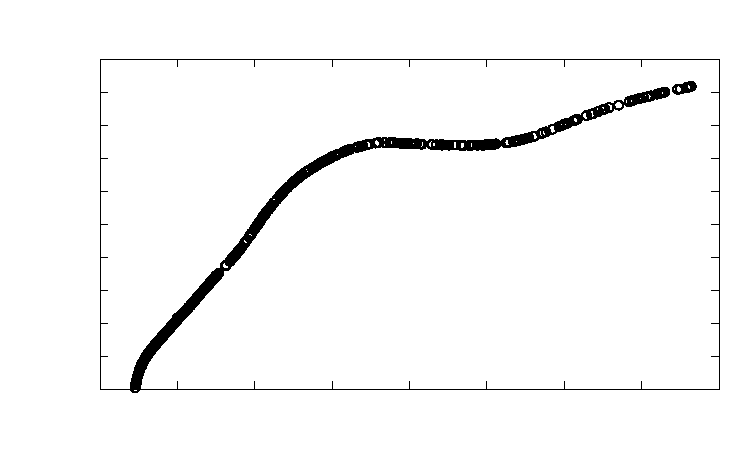
\includegraphics{GRAPH_color_graph3}}%
    \gplfronttext
  \end{picture}%
\endgroup

		% 			}\endgroup
		% 	\caption{Graph showing the colour-colour region for z=8.54-10.1. The colour window was defined as $Y-J{\ge}11.019$ and $J-H{\le}5.298$\label{fig:col3}}
		% \end{figure}
		% \begin{figure}[!htbp]
		% 	\centering
		% 		\begingroup\endlinechar=-1
		% 			\resizebox{0.7\textwidth}{!}{%
		% 				% GNUPLOT: LaTeX picture with Postscript
\begingroup
  \makeatletter
  \providecommand\color[2][]{%
    \GenericError{(gnuplot) \space\space\space\@spaces}{%
      Package color not loaded in conjunction with
      terminal option `colourtext'%
    }{See the gnuplot documentation for explanation.%
    }{Either use 'blacktext' in gnuplot or load the package
      color.sty in LaTeX.}%
    \renewcommand\color[2][]{}%
  }%
  \providecommand\includegraphics[2][]{%
    \GenericError{(gnuplot) \space\space\space\@spaces}{%
      Package graphicx or graphics not loaded%
    }{See the gnuplot documentation for explanation.%
    }{The gnuplot epslatex terminal needs graphicx.sty or graphics.sty.}%
    \renewcommand\includegraphics[2][]{}%
  }%
  \providecommand\rotatebox[2]{#2}%
  \@ifundefined{ifGPcolor}{%
    \newif\ifGPcolor
    \GPcolortrue
  }{}%
  \@ifundefined{ifGPblacktext}{%
    \newif\ifGPblacktext
    \GPblacktexttrue
  }{}%
  % define a \g@addto@macro without @ in the name:
  \let\gplgaddtomacro\g@addto@macro
  % define empty templates for all commands taking text:
  \gdef\gplbacktext{}%
  \gdef\gplfronttext{}%
  \makeatother
  \ifGPblacktext
    % no textcolor at all
    \def\colorrgb#1{}%
    \def\colorgray#1{}%
  \else
    % gray or color?
    \ifGPcolor
      \def\colorrgb#1{\color[rgb]{#1}}%
      \def\colorgray#1{\color[gray]{#1}}%
      \expandafter\def\csname LTw\endcsname{\color{white}}%
      \expandafter\def\csname LTb\endcsname{\color{black}}%
      \expandafter\def\csname LTa\endcsname{\color{black}}%
      \expandafter\def\csname LT0\endcsname{\color[rgb]{1,0,0}}%
      \expandafter\def\csname LT1\endcsname{\color[rgb]{0,1,0}}%
      \expandafter\def\csname LT2\endcsname{\color[rgb]{0,0,1}}%
      \expandafter\def\csname LT3\endcsname{\color[rgb]{1,0,1}}%
      \expandafter\def\csname LT4\endcsname{\color[rgb]{0,1,1}}%
      \expandafter\def\csname LT5\endcsname{\color[rgb]{1,1,0}}%
      \expandafter\def\csname LT6\endcsname{\color[rgb]{0,0,0}}%
      \expandafter\def\csname LT7\endcsname{\color[rgb]{1,0.3,0}}%
      \expandafter\def\csname LT8\endcsname{\color[rgb]{0.5,0.5,0.5}}%
    \else
      % gray
      \def\colorrgb#1{\color{black}}%
      \def\colorgray#1{\color[gray]{#1}}%
      \expandafter\def\csname LTw\endcsname{\color{white}}%
      \expandafter\def\csname LTb\endcsname{\color{black}}%
      \expandafter\def\csname LTa\endcsname{\color{black}}%
      \expandafter\def\csname LT0\endcsname{\color{black}}%
      \expandafter\def\csname LT1\endcsname{\color{black}}%
      \expandafter\def\csname LT2\endcsname{\color{black}}%
      \expandafter\def\csname LT3\endcsname{\color{black}}%
      \expandafter\def\csname LT4\endcsname{\color{black}}%
      \expandafter\def\csname LT5\endcsname{\color{black}}%
      \expandafter\def\csname LT6\endcsname{\color{black}}%
      \expandafter\def\csname LT7\endcsname{\color{black}}%
      \expandafter\def\csname LT8\endcsname{\color{black}}%
    \fi
  \fi
  \setlength{\unitlength}{0.0500bp}%
  \begin{picture}(7200.00,4320.00)%
    \gplgaddtomacro\gplbacktext{%
      \put(645,595){\makebox(0,0)[r]{\strut{} 10}}%
      \put(645,947){\makebox(0,0)[r]{\strut{} 15}}%
      \put(645,1299){\makebox(0,0)[r]{\strut{} 20}}%
      \put(645,1650){\makebox(0,0)[r]{\strut{} 25}}%
      \put(645,2002){\makebox(0,0)[r]{\strut{} 30}}%
      \put(645,2354){\makebox(0,0)[r]{\strut{} 35}}%
      \put(645,2706){\makebox(0,0)[r]{\strut{} 40}}%
      \put(645,3057){\makebox(0,0)[r]{\strut{} 45}}%
      \put(645,3409){\makebox(0,0)[r]{\strut{} 50}}%
      \put(645,3761){\makebox(0,0)[r]{\strut{} 55}}%
      \put(747,409){\makebox(0,0){\strut{} 0}}%
      \put(1515,409){\makebox(0,0){\strut{} 2}}%
      \put(2284,409){\makebox(0,0){\strut{} 4}}%
      \put(3052,409){\makebox(0,0){\strut{} 6}}%
      \put(3820,409){\makebox(0,0){\strut{} 8}}%
      \put(4588,409){\makebox(0,0){\strut{} 10}}%
      \put(5357,409){\makebox(0,0){\strut{} 12}}%
      \put(6125,409){\makebox(0,0){\strut{} 14}}%
      \put(6893,409){\makebox(0,0){\strut{} 16}}%
      \csname LTb\endcsname%
      \put(144,2178){\rotatebox{-270}{\makebox(0,0){\strut{}f150w-f200w}}}%
      \csname LTb\endcsname%
      \put(3820,130){\makebox(0,0){\strut{}f115w-f150w}}%
      \put(3820,4040){\makebox(0,0){\strut{}Redshift 10--14}}%
    }%
    \gplgaddtomacro\gplfronttext{%
    }%
    \gplbacktext
    \put(0,0){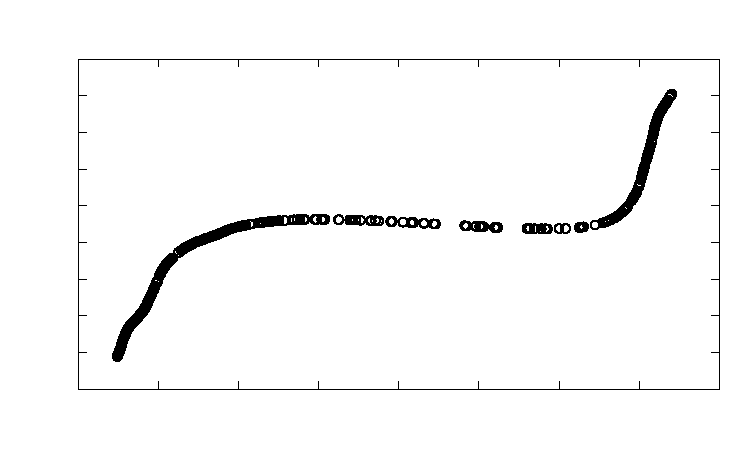
\includegraphics{GRAPH_color_graph4}}%
    \gplfronttext
  \end{picture}%
\endgroup

		% 			}\endgroup
		% 	\caption{Graph showing the colour-colour region for z=10-14. The colour window was defined as $f115w-f150w{\ge}14.439$ and $f150w-f200w{\le}14.815$\label{fig:col4}}
		% \end{figure}

	%subsection Results_for_Colour (end)

	\subsection{Interpretation of Colour Results}
	\label{sub:Interp_Colour}
		Constraining a colour window for observations turned out to be a challenging task. There are various errors that could make the results invalid and are discussed here.

	%section Interpetation_of_colour_results (end)

%section Photometry_and_colour (end)
